\chapter{Numerical results}
In order to quantify the results of the previous chapter it is usefull to parameterize the solutions of the rate equations above, especially the solution for the B-L asymmetry described by \eqref{eq:B-L_rate_expanding_interaction} or \eqref{eq:B-L_rate_expanding_interaction_rel} using the so called final efficiency factor $\kappa$ defined via
\begin{equation}
\lim\limits_{z\rightarrow\infty}\frac{n_{B-L}}{n_\gamma^{eq}}=\frac{3}{4}\epsilon\kappa,
\label{eq:efficiency}
\end{equation}
with $n_\gamma^{eq}=2\zeta(3)T^3/\pi^2$ the equilibrium density of photons and $\epsilon$ the CP-asymmetry parameter. It is now more convenient to rewrite the rate equations in terms of $N_i:=n_i/n_\gamma^{eq}$ with $i=B-L,N$. Using this substitution, one has to consider the transformation \cite[Eq. 7.1]{Wormann:2016yyi}
\begin{equation}
\frac{d}{dt}(N_in_\gamma^{eq})+3Hn_i=\frac{dN_i}{dt}n_\gamma^{eq}.
\end{equation}
Also, since the limit in \eqref{eq:efficiency} considers $z$ instead of the time $t$ one has to change the dependence from $t$ to $z$ by using
\begin{equation}
\frac{d}{dt}=\frac{dz}{dt}\frac{d}{z}=\frac{dz}{dT}\frac{dT}{dt}\frac{d}{dz}=-\frac{M_N}{T^2}\cdot(-HT)\frac{d}{dz}=zH\frac{d}{dz}.
\end{equation}
Combining all this results in the new, uncorrected rate equations
\begin{equation*}
zH\frac{dN_N}{dz}=\Gamma_0\left(N_N^{eq}-N_N\right),
\end{equation*}
\begin{equation*}
zH\frac{dN_{B-L}}{dz}=\Gamma_0\left[\epsilon\left(N_N-N_N^{eq}\right)+\frac{3}{\pi^2}\:\left(c_\ell+\frac{c_\phi}{2}\right)z^2K_1(z)N_{B-L}\right],
\end{equation*}
with $N_N^{eq}=3/8\:z^2K_2(z)$.
Now by dividing these rate equations by the factor $zH$ and by using \eqref{eq:washout} one finally arrives at
\begin{equation}
zH\frac{dN_N}{dz}=zK\left(N_N^{eq}-N_N\right),
\end{equation}
\begin{equation}
zH\frac{dN_{B-L}}{dz}=zK\left[\epsilon\left(N_N-N_N^{eq}\right)+\frac{3}{\pi^2}\:\left(c_\ell+\frac{c_\phi}{2}\right)z^2K_1(z)N_{B-L}\right],
\end{equation}\newpage
During the calculations of the coefficients in the rate equations, more precisely during the calculation of $\Gamma_{B-L}$ there were two occasions in which the explicit forms of particle distributions had to be used, namely for obtaining the equations \eqref{eq:chempot_l} and \eqref{eq:chempot_phi} and even before that for calculating the product $f_\ell f_\phi$. \newline \indent
In the first case quantum statistics were used for leptons and Higgses respectively, yielding the result given in that section. If one uses classical Boltzmann statistics the result changes by a seemingly not that impactful numerical coefficient of 12/$\pi^2$, yielding
\begin{equation}
\Gamma\textsubscript{B-L}=\frac{1}{4}\:\left(c_\ell+\frac{c_\phi}{2}\right)z^2K_1(z)\Gamma_0,
\label{eq:Gamma_B-l_classical}
\end{equation}
as given in appendix \ref{ap:statistics}.
\begin{figure}[H]
	\centering
	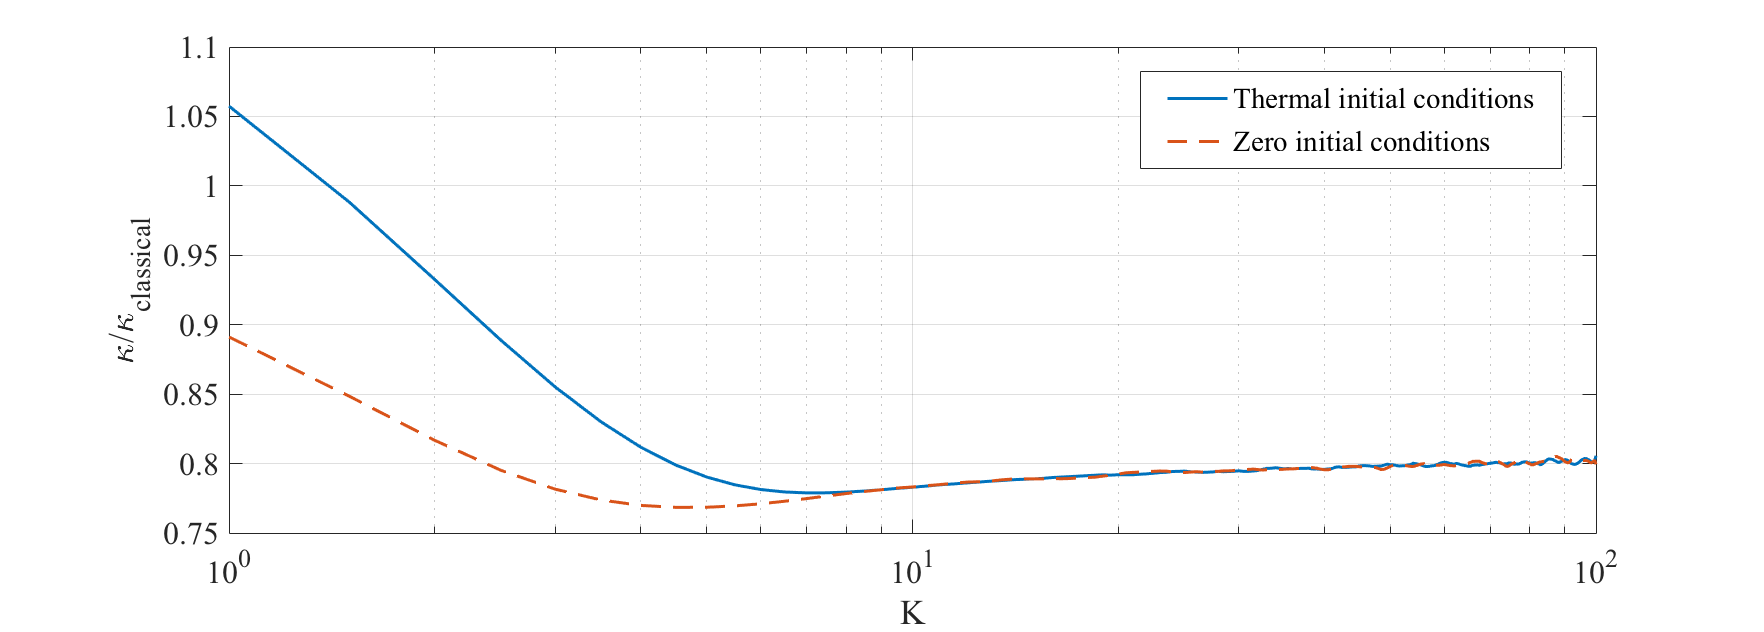
\includegraphics[width=0.8\linewidth]{Images/quantum}
	\caption{The final efficiency factor determined using the respective quantum stastics to obtain equations for the chemical potentials of leptons and Higgses normalized by the final efficiency factor obtained by using classical Boltzmann statistics for thermal and vanishing initial conditions. $c_l=1$ and $c_\phi=0$ were used.}
	\label{fig:quantum}
\end{figure} \noindent
Figure \ref{fig:quantum} however clearly shows that using Boltzmann statistics drasticly changes the final efficiency factor. For small K and thermal initial conditions the classical approximation is about 5\% smaller than the result obtained using quantum statistics, while for zero initial conditions the classical approximation exeeds the quantum calculation by $\sim$12\%. For growing K the classical approximation grows larger, surpassing the quantum calculation more and more and the deviation peaks at about 24\% for K $\simeq$ 4 and zero initial conditions and at about 22\% for K $\simeq$ 7.5 and thermal initial conditions, respetively. For an even larger wash out parameter this deviation slightly lowers until it reaches around 20\% for K$\simeq$ 50 for both sets of initial conditions. From this point on $\kappa/\kappa_{classical}$ practically stays constant for growing K.
This clearly highlights the importance of using the right statistics, as using classical statistics is a somewhat good approximation only for small wash out parameters, while it completly fails for higher wash out parameters.\newline \indent
On the other hand, because the Higgs particles and leptons are of high energy and the corresponding integrals don't saturate at momenta of order T they can be treated using Maxwell-Boltzmann statistics, in order to calculate the quantity $f_\ell f_\phi-f_{\bar{\ell}}f_{\bar{\phi}}$. Nevertheless it is interesting to see how using the correct quantum statistics and therefore not neglecting their quantum characteristics, affect previous results
As also shown in appendix \ref{ap:statistics}, this leads the following correction of the coefficient $\Gamma_{B-L}$
\begin{equation}
\Gamma_{B-L}=\frac{3}{\pi^2}\:z^3\left(\frac{e^{z/2}}{e^{z/2}-1}\:\frac{c_\phi}{2}+\frac{e^{z/2}}{e^{z/2}-1}c_\ell\right)\int_{1}^{\infty}dx\frac{\sqrt{x^2-1}}{e^{zx}-1}\Gamma_0
\label{eq:B-L_corrected}
\end{equation}
\begin{figure}[H]
	\centering
	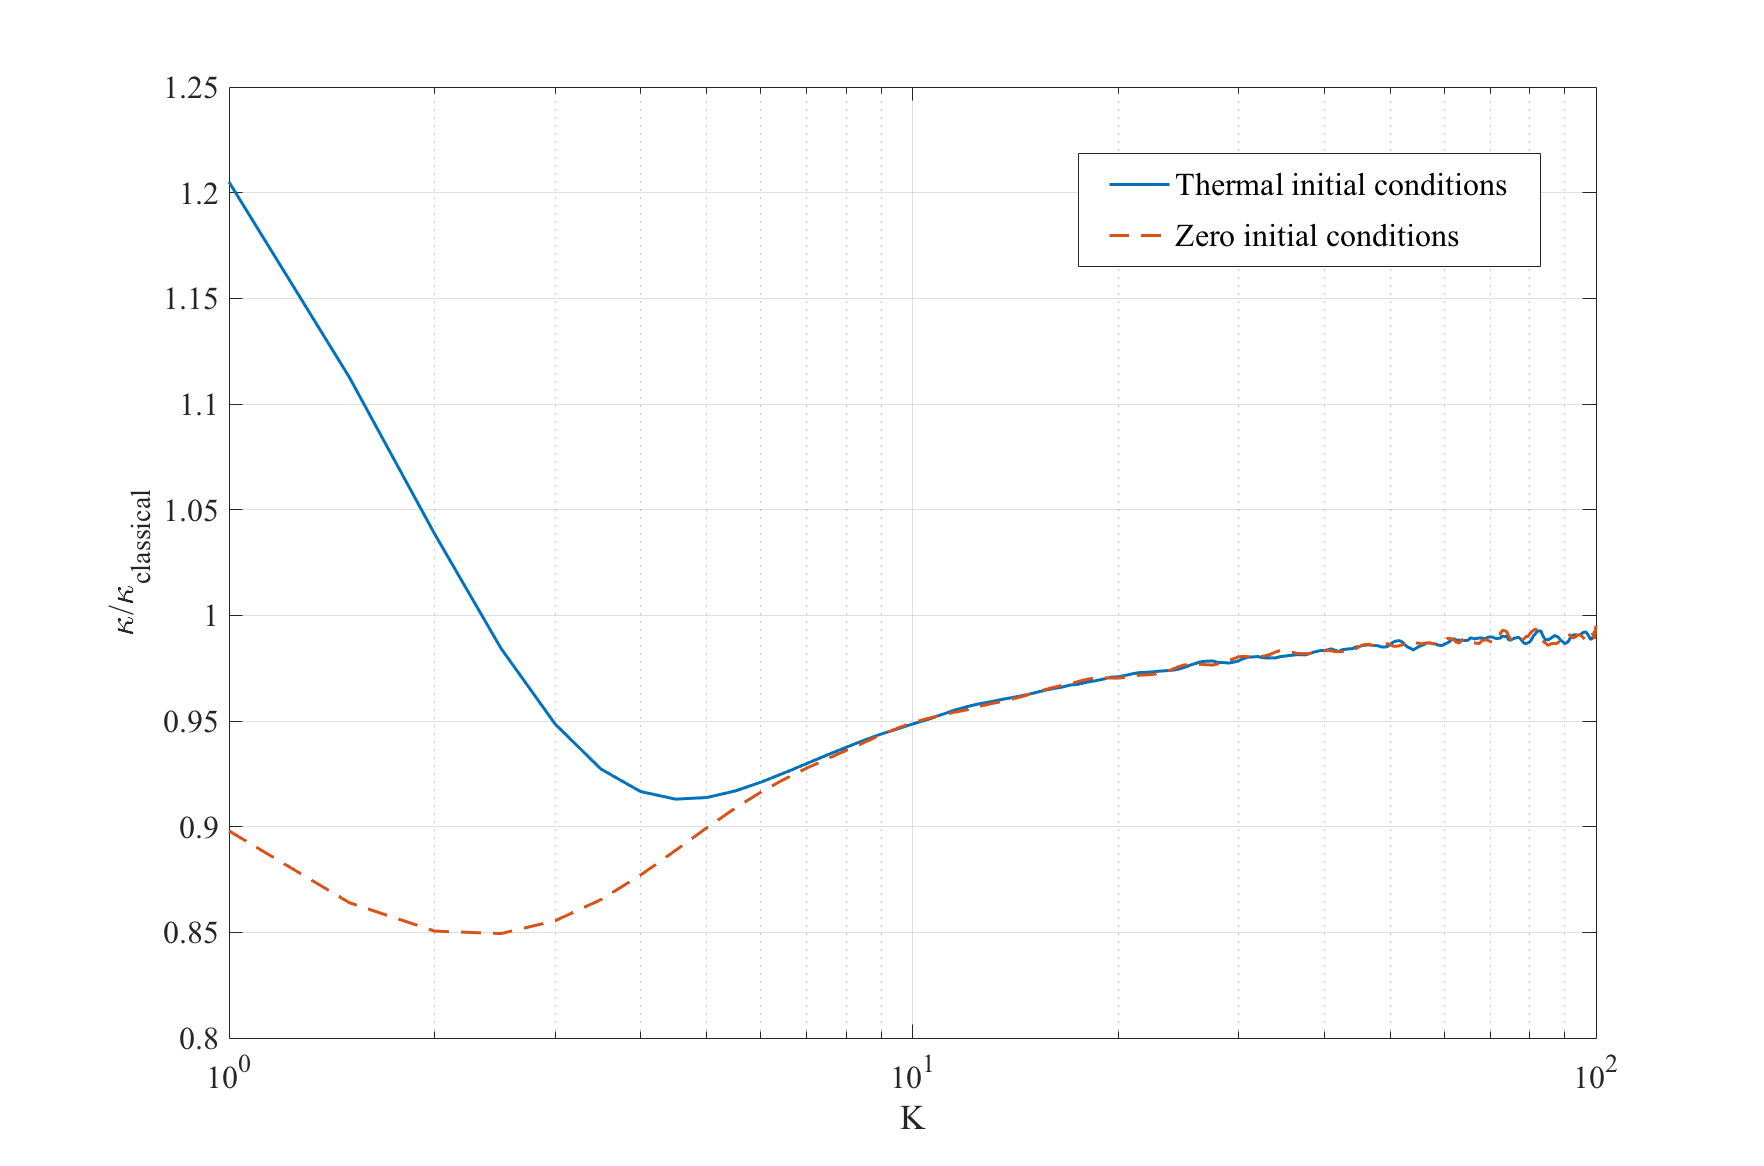
\includegraphics[width=0.8\linewidth]{Images/quantum1}
	\caption{The final efficiency factor determined using only the respective quantum stastics for obtaining $f_\ell f_\phi$ normalized by the final efficiency factor obtained by using classical Boltzmann statistics for thermal and vanishing initial conditions. $c_l=1$ and $c_\phi=0$ were used.}
	\label{fig:quantum1}
\end{figure} \noindent
Figure \ref{fig:quantum1} shows how using \eqref{eq:B-L_corrected} instead of \eqref{eq:Gamma_B-l_result} affects the final efficency factor. In the general the course of the graphs is similar to the ones in figure \ref{fig:quantum}, however the differences lie in the reached values of the derivation. For K$\sim$1 $\kappa_{classical}$ is about 20\% greater than $\kappa$ for thermal initial conditions and therefore the deviation here is bigger as in \ref{fig:quantum}. For zero initial conditions on the other hand the deviation of about 13\% is comparable to the one above. Now $\kappa_{classical}$ grows bigger with K and surpasses, if not already the case, $\kappa$ but the drop of $\kappa/\kappa_{classical}$ is not severe as above, as it peaks at around 82\% for zero initial conditions and K$\sim$ 2, meaning $\kappa_{classical}$ is about 18\% bigger than $\kappa$. For thermal initial conditions this effect is even smaller with the discrepancy between the to efficiency factor reaching its maximum at around 91\%. For both sets of initial conditions this effect gets smaller with growing K, so at K=50, the point where a nearly constant difference of about 20\% sets in above, the difference is below 2\%. \newline \indent
This is a clear sign showing that in the latter of the cases mentioned above using a classical approximation can have a meaningfull impact on the final efficiency for a low wash out parameter, but it slowly gets neglectable for higher K in contrast to the first case where the discrepancy between classical and quanum statistics is about 20\% even for high K.